% =====================================================================
% Research Methodology Architecture Diagram (Phase 2) -- DMT-GNN
% Standalone TikZ source. Compile with:  pdflatex methodology_architecture.tex
% The resulting methodology_architecture.pdf is included by cn_phase2.tex.
% Every box is labelled with the methodology step (Section 10) it implements.
% =====================================================================
\documentclass[tikz,border=4pt]{standalone}
\usepackage[T1]{fontenc}
\usepackage{lmodern}
\usepackage{amsmath,amssymb}
\usetikzlibrary{arrows.meta,positioning,calc,fit,backgrounds}
\renewcommand{\familydefault}{\sfdefault}

\definecolor{cData}{HTML}{2B6CB0}
\definecolor{cPrep}{HTML}{4A5568}
\definecolor{cModel}{HTML}{C05621}
\definecolor{cBase}{HTML}{2F855A}
\definecolor{cExp}{HTML}{6B46C1}
\definecolor{cEval}{HTML}{B7791F}
\definecolor{cOut}{HTML}{1A202C}

\tikzset{
  box/.style={draw=#1, fill=#1!9, rounded corners=2.5pt, line width=0.7pt,
              align=center, font=\sffamily\footnotesize, inner sep=3pt,
              text=black},
  hdr/.style={font=\sffamily\bfseries\footnotesize, text=#1},
  arr/.style={-{Stealth[length=2.4mm,width=1.8mm]}, line width=0.75pt, draw=black!65},
  darr/.style={arr, dashed},
  band/.style={draw=black!35, dashed, rounded corners=4pt, line width=0.5pt},
  bandlbl/.style={font=\sffamily\bfseries\scriptsize, text=black!60, anchor=north west,
                  fill=white, inner sep=1.5pt},
  lbl/.style={font=\sffamily\scriptsize, text=black!75}
}
% Band titles are drawn on a foreground layer so that arrows pass beneath them.
\pgfdeclarelayer{foreground}
\pgfsetlayers{main,foreground}

\begin{document}
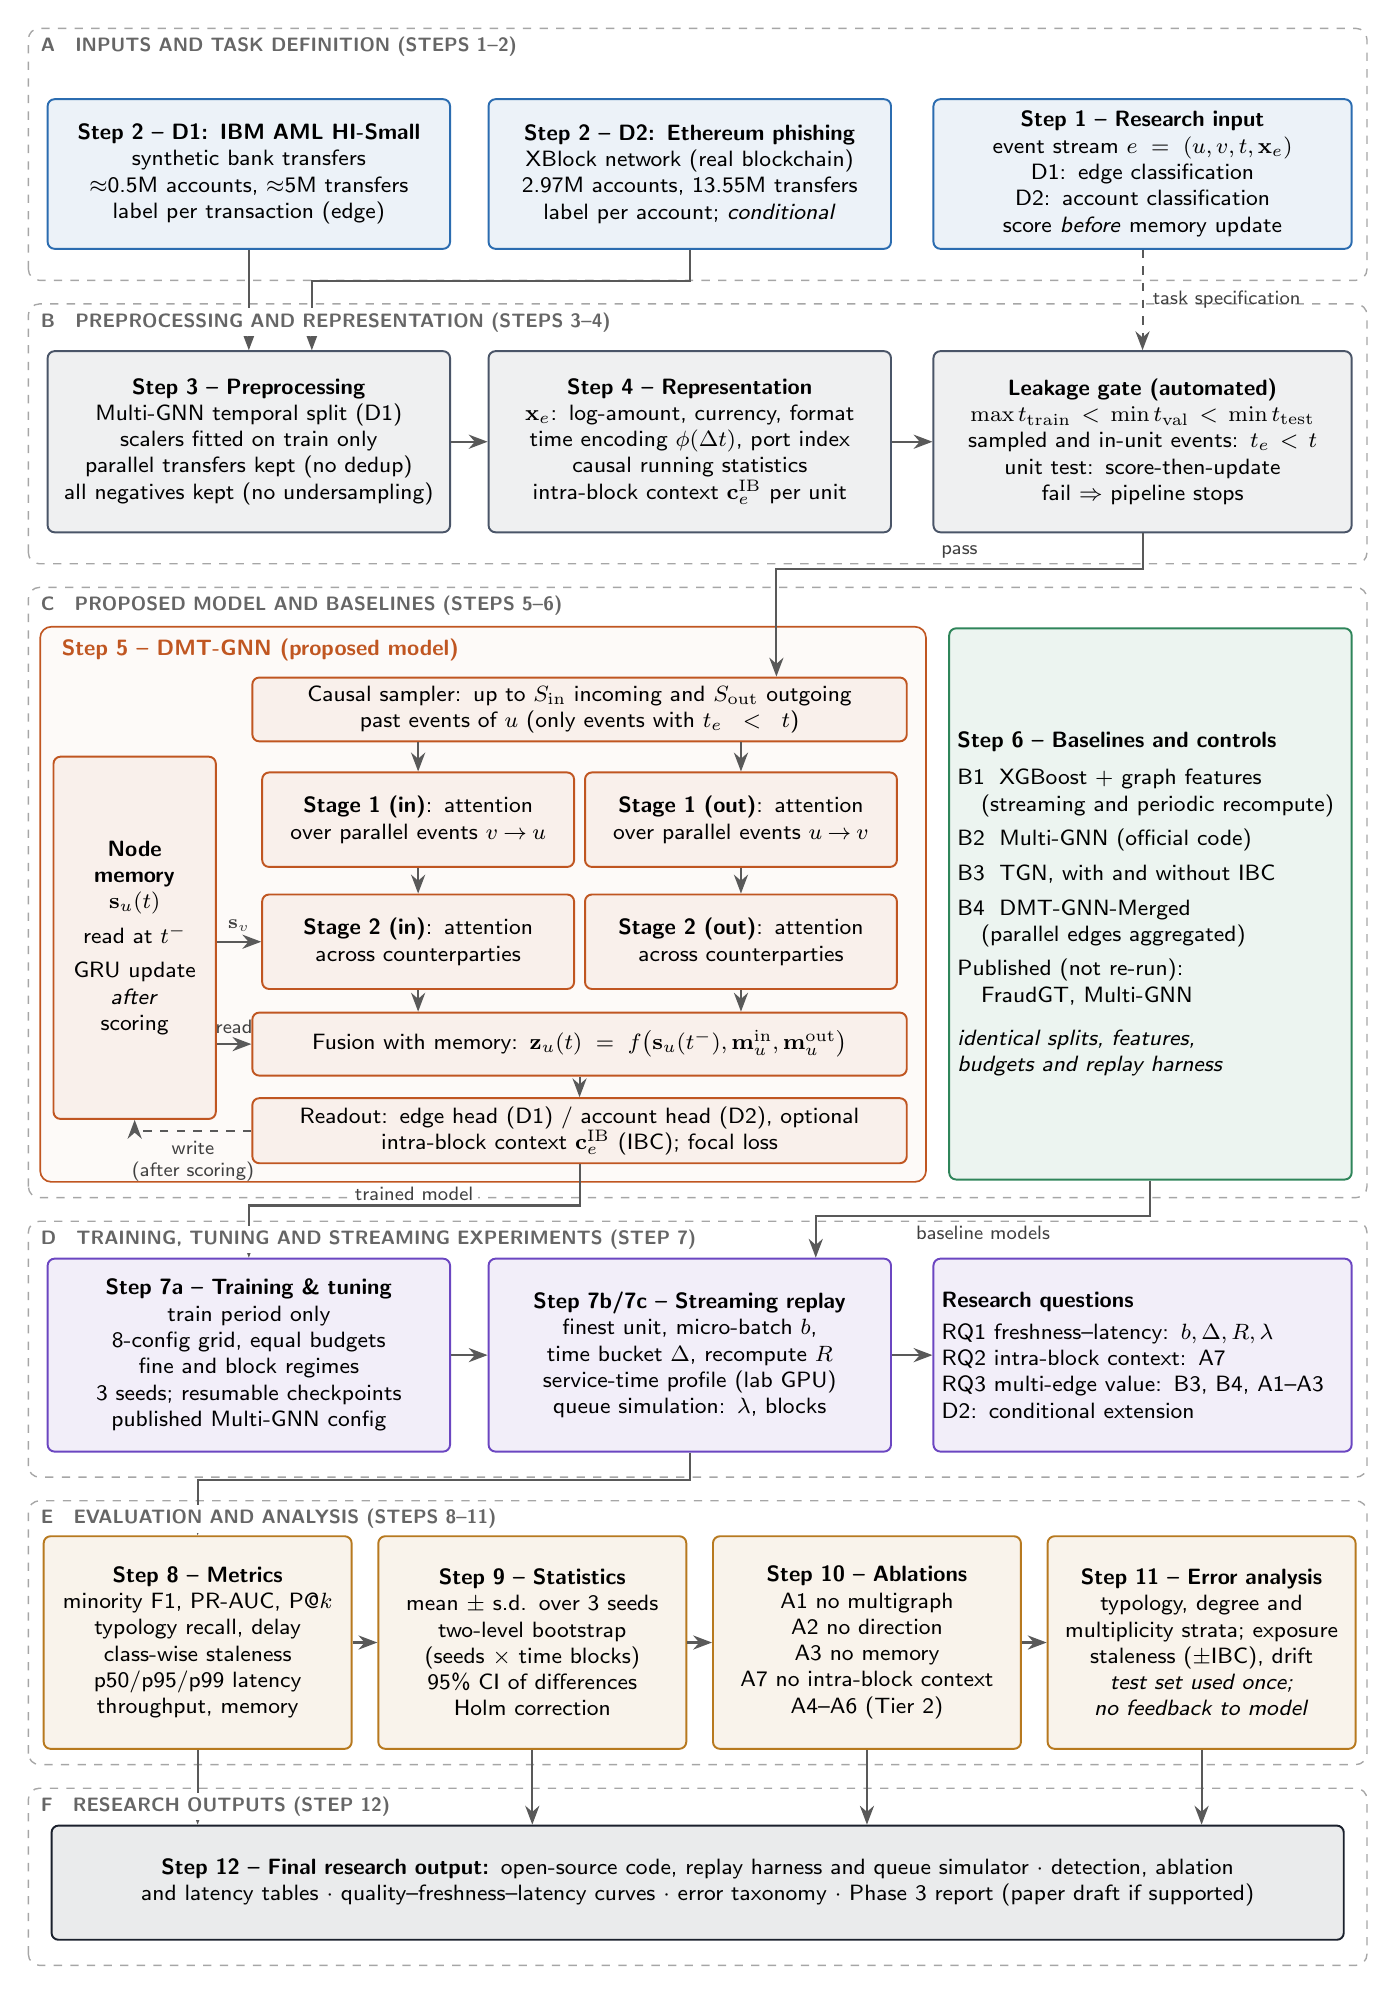
\begin{tikzpicture}[x=1cm,y=1cm]

% ------------------------------------------------------------- bands
\draw[band] (0,21.4) rectangle (17.0,24.6);
\draw[band] (0,17.8) rectangle (17.0,21.1);
\draw[band] (0,9.75) rectangle (17.0,17.5);
\draw[band] (0,6.2) rectangle (17.0,9.45);
\draw[band] (0,2.55) rectangle (17.0,5.9);
\draw[band] (0,0.0) rectangle (17.0,2.25);
\begin{pgfonlayer}{foreground}
\node[bandlbl] at (0.1,24.55) {A \; INPUTS AND TASK DEFINITION (STEPS 1--2)};
\node[bandlbl] at (0.1,21.05) {B \; PREPROCESSING AND REPRESENTATION (STEPS 3--4)};
\node[bandlbl] at (0.1,17.45) {C \; PROPOSED MODEL AND BASELINES (STEPS 5--6)};
\node[bandlbl] at (0.1,9.4) {D \; TRAINING, TUNING AND STREAMING EXPERIMENTS (STEP 7)};
\node[bandlbl] at (0.1,5.85) {E \; EVALUATION AND ANALYSIS (STEPS 8--11)};
\node[bandlbl] at (0.1,2.2) {F \; RESEARCH OUTPUTS (STEP 12)};
\end{pgfonlayer}

% ------------------------------------------------------------- band A
\node[box=cData, text width=4.9cm, minimum height=1.9cm] (d1) at (2.8,22.75)
  {\textbf{Step 2 -- D1: IBM AML HI-Small}\\ synthetic bank transfers\\ $\approx$0.5M accounts, $\approx$5M transfers\\ label per transaction (edge)};
\node[box=cData, text width=4.9cm, minimum height=1.9cm] (d2) at (8.4,22.75)
  {\textbf{Step 2 -- D2: Ethereum phishing}\\ XBlock network (real blockchain)\\ 2.97M accounts, 13.55M transfers\\ label per account; \emph{conditional}};
\node[box=cData, text width=5.1cm, minimum height=1.9cm] (task) at (14.15,22.75)
  {\textbf{Step 1 -- Research input}\\ event stream $e=(u,v,t,\mathbf{x}_e)$\\ D1: edge classification\\ D2: account classification\\ score \emph{before} memory update};

% ------------------------------------------------------------- band B
\node[box=cPrep, text width=4.9cm, minimum height=2.3cm] (prep) at (2.8,19.35)
  {\textbf{Step 3 -- Preprocessing}\\ Multi-GNN temporal split (D1)\\ scalers fitted on train only\\ parallel transfers kept (no dedup)\\ all negatives kept (no undersampling)};
\node[box=cPrep, text width=4.9cm, minimum height=2.3cm] (repr) at (8.4,19.35)
  {\textbf{Step 4 -- Representation}\\ $\mathbf{x}_e$: log-amount, currency, format\\ time encoding $\phi(\Delta t)$, port index\\ causal running statistics\\ intra-block context $\mathbf{c}^{\mathrm{IB}}_e$ per unit};
\node[box=cPrep, text width=5.1cm, minimum height=2.3cm] (gate) at (14.15,19.35)
  {\textbf{Leakage gate (automated)}\\ $\max t_{\mathrm{train}}<\min t_{\mathrm{val}}<\min t_{\mathrm{test}}$\\ sampled and in-unit events: $t_e<t$\\ unit test: score-then-update\\ fail $\Rightarrow$ pipeline stops};

% ------------------------------------------------------------- band C (model)
\draw[draw=cModel, rounded corners=4pt, line width=0.6pt, fill=cModel!3] (0.15,9.95) rectangle (11.4,17.0);
\node[hdr=cModel, anchor=west] at (0.3,16.7) {Step 5 -- DMT-GNN (proposed model)};
\node[box=cModel, text width=8.1cm, minimum height=0.8cm] (samp) at (7.0,15.95)
  {Causal sampler: up to $S_{\mathrm{in}}$ incoming and $S_{\mathrm{out}}$ outgoing\\ past events of $u$ (only events with $t_e<t$)};
\node[box=cModel, text width=3.75cm, minimum height=1.2cm] (s1i) at (4.95,14.55)
  {\textbf{Stage 1 (in)}: attention over parallel events $v\!\rightarrow\!u$};
\node[box=cModel, text width=3.75cm, minimum height=1.2cm] (s1o) at (9.05,14.55)
  {\textbf{Stage 1 (out)}: attention over parallel events $u\!\rightarrow\!v$};
\node[box=cModel, text width=3.75cm, minimum height=1.2cm] (s2i) at (4.95,13.0)
  {\textbf{Stage 2 (in)}: attention across counterparties};
\node[box=cModel, text width=3.75cm, minimum height=1.2cm] (s2o) at (9.05,13.0)
  {\textbf{Stage 2 (out)}: attention across counterparties};
\node[box=cModel, text width=8.1cm, minimum height=0.8cm] (fuse) at (7.0,11.7)
  {Fusion with memory: $\mathbf{z}_u(t)=f\big(\mathbf{s}_u(t^-),\mathbf{m}^{\mathrm{in}}_u,\mathbf{m}^{\mathrm{out}}_u\big)$};
\node[box=cModel, text width=8.1cm, minimum height=0.8cm] (head) at (7.0,10.6)
  {Readout: edge head (D1) / account head (D2), optional\\ intra-block context $\mathbf{c}^{\mathrm{IB}}_e$ (IBC); focal loss};
\node[box=cModel, text width=1.85cm, minimum height=4.6cm] (mem) at (1.35,13.05)
  {\textbf{Node}\\ \textbf{memory}\\ $\mathbf{s}_u(t)$\\[3pt] read at $t^-$\\[3pt] GRU update\\ \emph{after}\\ scoring};

\draw[arr] (samp.south -| s1i) -- (s1i.north);
\draw[arr] (samp.south -| s1o) -- (s1o.north);
\draw[arr] (s1i) -- (s2i);
\draw[arr] (s1o) -- (s2o);
\draw[arr] (s2i.south) -- (s2i.south |- fuse.north);
\draw[arr] (s2o.south) -- (s2o.south |- fuse.north);
\draw[arr] (fuse) -- (head);
\draw[arr] (mem.east |- fuse) -- (fuse.west) node[midway,above,lbl]{read};
\draw[arr] (mem.east |- s2i) -- (s2i.west) node[midway,above,lbl]{$\mathbf{s}_v$};
\draw[darr] (head.west) -| (mem.south) node[pos=0.25,below,lbl,align=center]{write\\(after scoring)};

% ------------------------------------------------------------- band C (baselines)
\node[box=cBase, text width=4.9cm, minimum height=7.0cm, align=left] (base) at (14.25,13.48)
  {\textbf{Step 6 -- Baselines and controls}\\[4pt]
   B1\; XGBoost + graph features\\ \quad (streaming and periodic recompute)\\[3pt]
   B2\; Multi-GNN (official code)\\[3pt]
   B3\; TGN, with and without IBC\\[3pt]
   B4\; DMT-GNN-Merged\\ \quad (parallel edges aggregated)\\[3pt]
   Published (not re-run):\\ \quad FraudGT, Multi-GNN\\[6pt]
   \textit{identical splits, features,}\\ \textit{budgets and replay harness}};

% ------------------------------------------------------------- band D
\node[box=cExp, text width=4.9cm, minimum height=2.45cm] (train) at (2.8,7.75)
  {\textbf{Step 7a -- Training \& tuning}\\ train period only\\ 8-config grid, equal budgets\\ fine and block regimes\\ 3 seeds; resumable checkpoints\\ published Multi-GNN config};
\node[box=cExp, text width=4.9cm, minimum height=2.45cm] (harn) at (8.4,7.75)
  {\textbf{Step 7b/7c -- Streaming replay}\\ finest unit, micro-batch $b$,\\ time bucket $\Delta$, recompute $R$\\ service-time profile (lab GPU)\\ queue simulation: $\lambda$, blocks};
\node[box=cExp, text width=5.1cm, minimum height=2.45cm, align=left] (rq) at (14.15,7.75)
  {\textbf{Research questions}\\[2pt]
   RQ1 freshness--latency: $b,\Delta,R,\lambda$\\
   RQ2 intra-block context: A7\\
   RQ3 multi-edge value: B3, B4, A1--A3\\
   D2: conditional extension};

% ------------------------------------------------------------- band E
\node[box=cEval, text width=3.7cm, minimum height=2.7cm] (met) at (2.15,4.1)
  {\textbf{Step 8 -- Metrics}\\ minority F1, PR-AUC, P@$k$\\ typology recall, delay\\ class-wise staleness\\ p50/p95/p99 latency\\ throughput, memory};
\node[box=cEval, text width=3.7cm, minimum height=2.7cm] (sta) at (6.4,4.1)
  {\textbf{Step 9 -- Statistics}\\ mean $\pm$ s.d. over 3 seeds\\ two-level bootstrap\\ (seeds $\times$ time blocks)\\ 95\% CI of differences\\ Holm correction};
\node[box=cEval, text width=3.7cm, minimum height=2.7cm] (abl) at (10.65,4.1)
  {\textbf{Step 10 -- Ablations}\\ A1 no multigraph\\ A2 no direction\\ A3 no memory\\ A7 no intra-block context\\ A4--A6 (Tier 2)};
\node[box=cEval, text width=3.7cm, minimum height=2.7cm] (err) at (14.9,4.1)
  {\textbf{Step 11 -- Error analysis}\\ typology, degree and multiplicity strata; exposure\\ staleness ($\pm$IBC), drift\\ \emph{test set used once;}\\ \emph{no feedback to model}};

% ------------------------------------------------------------- band F
\node[box=cOut, text width=16.2cm, minimum height=1.45cm] (out) at (8.5,1.05)
  {\textbf{Step 12 -- Final research output:} open-source code, replay harness and queue simulator $\cdot$ detection, ablation and latency tables $\cdot$ quality--freshness--latency curves $\cdot$ error taxonomy $\cdot$ Phase 3 report (paper draft if supported)};

% ------------------------------------------------------------- inter-band arrows
\draw[arr] (d1) -- (prep);
\draw[arr] (d2.south) -- ++(0,-0.4) -| ([xshift=8mm]prep.north);
\draw[arr] (prep) -- (repr);
\draw[arr] (repr) -- (gate);
\draw[darr] (task) -- (gate) node[midway,right,lbl]{task specification};
\draw[arr] (gate.south) -- ++(0,-0.45) -| ([xshift=25mm]samp.north) node[pos=0.25,above,lbl]{pass};
\draw[arr] (head.south) -- (7.0, 9.65) -- (2.8, 9.65)
  node[midway, above, lbl, fill=white, inner sep=1.5pt] {trained model}
  -- (train.north);
\draw[arr] (base.south) -- ++(0,-0.45) -| ([xshift=16mm]harn.north) node[pos=0.25,below,lbl]{baseline models};
\draw[arr] (train) -- (harn);
\draw[arr] (harn) -- (rq);
\draw[arr] (harn.south) -- ++(0,-0.35) -| (met.north);
\draw[arr] (met) -- (sta);
\draw[arr] (sta) -- (abl);
\draw[arr] (abl) -- (err);
\foreach \n in {met,sta,abl,err} {\draw[arr] (\n.south) -- (\n.south |- out.north);}

\end{tikzpicture}
\end{document}
